\documentclass[10pt,aspectratio=169]{beamer}
\usetheme{default}

\setbeamercovered{invisible}
\setbeamertemplate{navigation symbols}{}
\setbeamertemplate{footline}{
    \flushright{\hfill \insertframenumber{}/\inserttotalframenumber}
}
\usepackage{listings}


\begin{document}
    \title{A discrete (stochastical)\protect\\SIR epidemiological model}
    \author{Matteo Caldana}
    \date{16/03/2023}
    
\begin{frame}[plain, noframenumbering]
    \maketitle
\end{frame}

\begin{frame}{Epidemiological model\footnote{This exercise is inspired by models shown in \\
\url{https://www.washingtonpost.com/graphics/2020/world/corona-simulator/} and \\
\url{https://github.com/seismotologist/coronaVirusContagion}.}}

Consider a discrete population of agents living in a 2D square domain.

\begin{figure}
    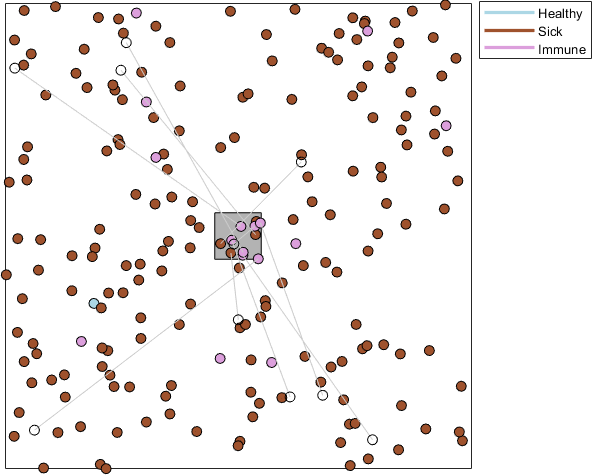
\includegraphics[width=0.5\textwidth]{contagion.png}
\end{figure}
\end{frame}

\begin{frame}{Contagion model}
Starting from random initial positions, the population evolves according to the following rules:

\begin{enumerate}
    \item Each agent can be either Susceptible to a virus, Infected or Recovered;
    \item At each timestep agents move randomly of a given step length;
    \item A prescribed percentage of agents does \textbf{social distancing}, \textit{i.e.} does not move, excepted the following rule;
    \item Each agent (\textit{i.e.} including those who do social distancing) goes to a pub placed at the center of the domain once every a fixed number of time steps;
    \item A agent is infected when close to another infected agent and recovers after a fixed number of time steps.
\end{enumerate}
\end{frame}

\begin{frame}{Exercise - Part 1}
Starting from the given files, start by implementing a \texttt{C++} program that simulates a simplified model such that
    \begin{enumerate}
        \item Exports the total number of susceptible, infected and recovered agents at each timestep to a \texttt{.csv} file (implement \texttt{Contagion::output\_results}).
        \item Exports the positions of each agent at each timestep, use a parameter to set the frequency of the export (implement inside \texttt{Contagion::run}).
        \item Use an \texttt{enum class} to define the possible agents states.
        \item Each \texttt{Agent} moves at random (implement a \texttt{Agent::move} method). Check that the agent stays in the domain, change the direction of the movement otherwise.
        \item The simulation is managed by the method \texttt{Contagion::run} which at each timestep
        \begin{enumerate}
            \item moves each agent
            \item checks the distance between agents, if one is Infected and the other Susceptible and they are close, than they become Infected
            \item counts the number of agents in each state
        \end{enumerate}
    \end{enumerate}
\end{frame}

\begin{frame}{Exercise - Part 2}
    \begin{enumerate}
        \item Performs the simulation employing the \texttt{<algorithm>} library and parallelize the code using the \texttt{<execution>} library where possible;
        \item Make the model more accurate by completing the \texttt{Agent::move} method following the ``Contagion model" slide. Use an \texttt{enum class} to define the possible agents actions.
    \end{enumerate}
\end{frame}

\begin{frame}{Cache aligment}
    Modern processors use a variety of techniques for performance. Caches is small amount of fast memory where values are ``cached" in hope of reusing recently used or nearby data.
    \begin{figure}
        \centering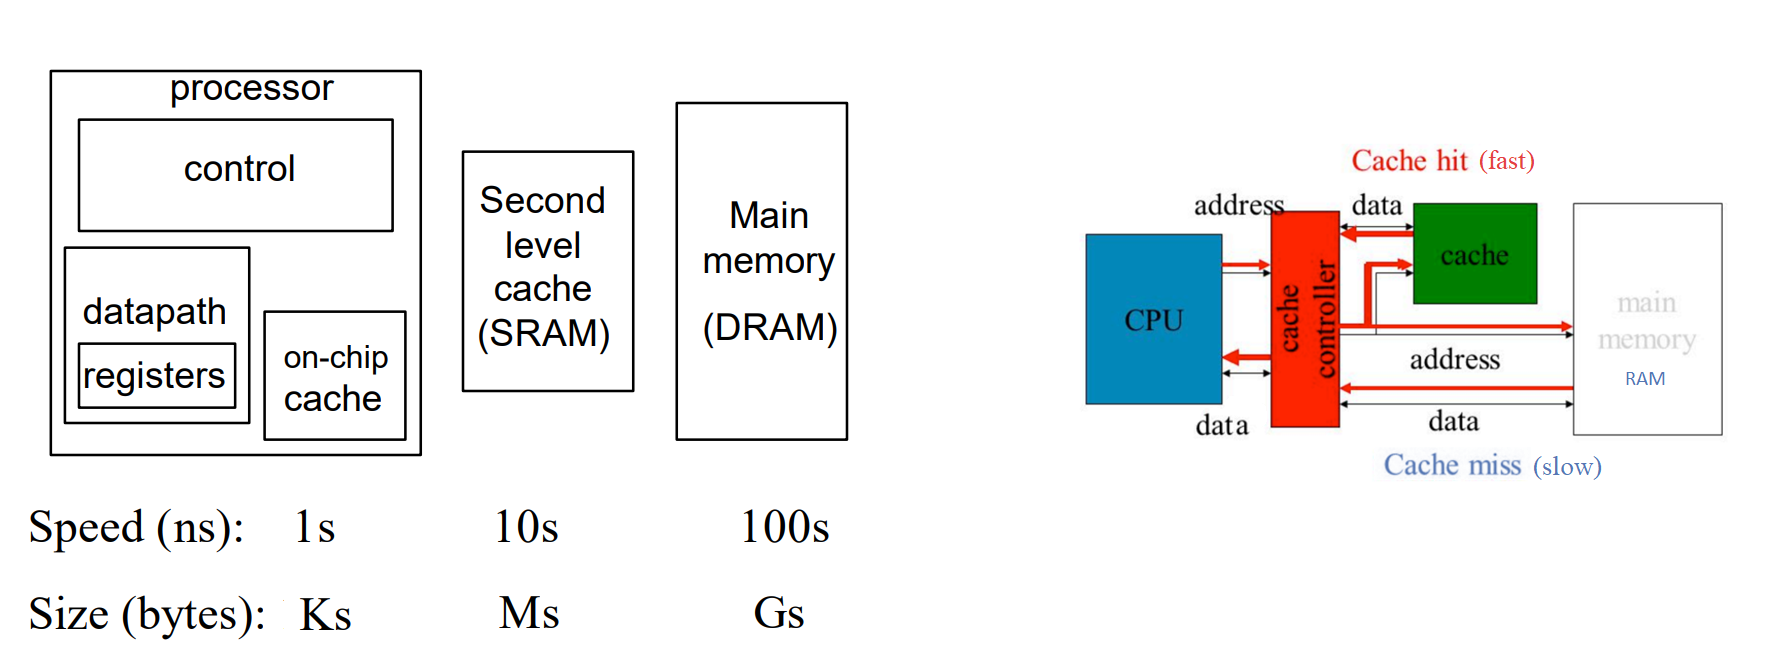
\includegraphics[width=0.8\textwidth]{cache.png}
    \end{figure}
    \begin{itemize}
        \item Taking into account cache aligment is key for linear algebra routines
        \item Libraries like \href{https://github.com/xianyi/OpenBLAS}{OpenBLAS} (which is among the mk modules) or ATLAS are tuned at compile time to take into account hardware specific parameters (like cache size).
        \item \texttt{-O3} aggressive compiler optimization option sometimes is able to do this
    \end{itemize}
\end{frame}

\begin{frame}{Exercise - Part 3}
    Let L1CS be the cache size of a CPU and let $v$ be a large vector of size $K\cdot$L1CS. Consider:
    \lstinputlisting[basicstyle=\footnotesize]{ex1.cpp}
    \begin{itemize}
        \item Optimize the cache alignment for the double for loop used for the radius checking step of the (sequential) simulation.
        \item Use \texttt{getconf -a | grep CACHE} to check the cache size of your PC.
        \item Confront the execution time for different number of agents between the two algorithms.
    \end{itemize}
\end{frame}

\begin{frame}{Possible extensions (homework)}
\begin{enumerate}
    \item Plot the curve of susceptible, infected and recovered using Python, you can read the \texttt{.csv} using the pandas module. You may need to install the matplotlib module with \texttt{pip install matplotlib}.
    \item Create an animation of the positions of the agents at each timestep using Python.
    \item Personalize agent-specific parameters, \textit{e.g.}
    \begin{itemize}
        \item by random generation, or
        \item by reading multiple pairs of \{agent index, parameter value\}\\
              for each parameter from file;
    \end{itemize}
    \item Take birth and mortality rates into account.
    \item Extend the model to 3D domains (possibly using templates).
\end{enumerate}
\end{frame}
\end{document}
